\documentclass[11]{beamer}
\usetheme{Warsaw}
\usepackage[utf8]{inputenc}
\usepackage{amsmath}
\usepackage{amsfonts}
\usepackage{amssymb}
\usepackage{color}
\usepackage{siunitx}
%\usepackage[table]{xcolor} 
\usepackage{color, colortbl}

\definecolor{LightCyan}{rgb}{0.88,1,1}
\definecolor{lightgray}{gray}{0.9}
\usepackage{tikz}
\usetikzlibrary{shapes,snakes,arrows,positioning}


% Define box and box title style
\tikzstyle{mybox} = [draw=red, fill=blue!20, very thick,
    rectangle, rounded corners, inner sep=10pt, inner ysep=20pt]
\tikzstyle{fancytitle} =[fill=red, text=white]

\author{Arindam BASU \hspace{5 cm}\newline{arindam@barc.gov.in}}
\title{Accelerator Technology-Vacuum \newline{Vacuum Introduction Part-1}}

%\setbeamercovered{transparent} 
%\setbeamertemplate{navigation symbols}{} 
%\logo{} 
\institute{IADD,BARC} 
%\date{} 
\subject{Accelerator Technology-Vacuum} 
\begin{document}

\begin{frame}
\titlepage
\end{frame}

%\begin{frame}
%\tableofcontents
%\end{frame}


\begin{frame}{Vacuum Fundamentals}
\begin{block}{Vacuum Facts}
\begin{itemize}
\item Vacuum is the condition in a closed volume where pressure is less than the normal atmospheric pressure. 
\item To classify and measure the vacuum , it is very important to define the normal atmospheric pressure.
At $0^0 C$ or 273 K , atmospheric pressure is equal to the weight per unit area of  760 mm column of mercury.
\item In vacuum terminology 760 mm column of mercury is known as 760 Torr, in honour of Italian scientist Torricelli who first created vacuum. Thus 1 mm  of mercury column is equal to 1 Torr.
\end{itemize}
\end{block}



\end{frame}



\begin{frame}{Vacuum Depiction}
\begin{center}
\includegraphics[width=1.0\textwidth]{VacuumDepiction.png}
\end{center}

\end{frame}


\begin{frame}{Classification of Vacuum}
Vacuum can be classified in three broader categories. These are 
\begin{center}
\includegraphics[width=0.5\textwidth]{Vacuum_Scale.png}
\end{center}

\begin{block}{}
	\begin{itemize}
		\item  Rough Vacuum :  759 to $1x 10^{-3}$ Torr
		\item  High Vacuum   :  $1x 10^{-3}$ Torr to $1x 10^{-6}$  Torr
		\item  Ultrahigh Vacuum  :$1x 10^{-6}$  Torr to $1x 10^{-10}$ Torr
		\item  Extra High Vacuum : Less than $1x 10^{-10}$ Torr
	\end{itemize}

\end{block}

\end{frame}

\begin{frame}{Units of Vacuum}

\begin{itemize}
  \item As vacuum is a state of lower gas pressure so unit of pressure such as Pascal or bar can be used to measure and describe the vacuum. 
  \item Though occasionally vacuum is expressed in terms of Pascal or bar but there is a unit defined to express the vacuum only.
  \item Most frequently used unit in vacuum is Torr and milli Bar(mbar).
  \item One Torr is equal to 1 mm of mercury column. So Torr unit represent pressure in terms of height of mercury column.
\end{itemize}
     

 1 atm = 101325 Pascals 
  \hspace{1cm}          = 14.7 lbs/in2 \\
  \hspace{1cm}          = 760 mmHg (Torr)\\
  \hspace{1cm}          = 1013.25 mbar\\
  \hspace{1cm}          = 29.92 inHg\\
  \hspace{1cm}          = 10332.27 $\dfrac{kg}{m^2} $ \\



\end{frame}

\begin{frame}{Vacuum and Gas Laws}

\begin{itemize}
\item Vacuum is a gas condition , hence gas laws are applicable in the study of Vacuum.
\item The gas laws such as \emph{Avogadro’s law, Boyle’s Law, Charles law, Gay Lussacs’ Law, Dalton partial pressure law} and concept of \emph{mean free path} is important to \textbf{design} and \textbf{maintain} a vacuum system.
\end{itemize}



\end{frame}
 
\begin{frame}{Vacuum and Gas Laws}
	\begin{exampleblock}{Dalton Law of Partial Pressure}
	
		The total pressure of the mixture of the gases is the sum of each of the individual gas pressures in the mixture. Each individual gas 	        pressure in the mixture is called partial pressure.
	\end{exampleblock}

\includegraphics[width=0.5\textwidth]{dalton_law_of_partial_pressure.jpg}
\includegraphics[width=0.4\textwidth]{Air_Partial_Pressure.jpg}
\end{frame}


\begin{frame}{Vacuum and Gas Laws}

\begin{exampleblock}{Ideal Gas Law}

$PV=nRT $ \break
At constant temperature $P \propto n$ \break
To establish vacuum in a vessel it is rerquired to remove gas molecules from the system. A Vacuum pump establishes vacuum in the chamber by removing gas molecules from the chamber.

\end{exampleblock}



\end{frame}





\begin{frame}{Kinetic Picture of Gas Molecules}

 \begin{exampleblock}{Assumptions}
	
	\begin{itemize}
 		\item The volume of gas under consideration contains a large number of molecules and atoms – Statistical distribution applies.
 		\item Intermolecular distance is much higher than the diameter of the individual molecule.
 		\item Molecules exert no force on one another, except when they collide. All collisions are elastic (i.e. no internal excitation).
 		\item Molecules are in a constant state of motion, in all direction equally. They will travel in straight lines until they collide with a wall, or with one another.
	\end{itemize}
 
  \end{exampleblock}

\end{frame}



 \begin{frame}{Velocity Distribution of Gas Molecules}
  
 \begin{exampleblock}{Maxwell Bolzman Distribution of Gas Molecules}
  \begin{center}
    \includegraphics[width=0.8\textwidth]{MaxwellDistribution.png}
  \end{center}
 \end{exampleblock}

\end{frame}


\begin{frame}{Velocity Distribution of Gas Molecules}

\begin{center}
\includegraphics[width=0.5\textwidth]{MaxwellDistributionCurve.png}
\end{center}

	\begin{exampleblock}

       \begin{itemize}
       \item Velocity Distribution is given by $f(v) = \left(\frac{m}{2 \pi kT}\right)^{\dfrac{3}{2}}\, 4\pi v^2 \exp \left(\frac{-mv^2}{2kT}\right)$
       \item Most probable speed $v_p =\sqrt{\dfrac{2kT}{m}}$ m/sec
        \item R.M.S speed $v_{rms} =\sqrt{\dfrac{3kT}{m}}=158\sqrt{\dfrac{T}{m}}$ m/sec
        \item Arithmetic Average speed $v_{a} =\sqrt{\dfrac{8kT}{\pi m}}=145.51\sqrt{\dfrac{T}{m}}$ m/sec
        
       \end{itemize}


	\end{exampleblock}

\end{frame}


\begin{frame}{Velocity Distribution of Gas Molecules}





 \begin{columns}[t]
    
      
   \column{0.5\textwidth}
       \begin{exampleblock}{Temperature Dependence}
         \begin{center}
			\includegraphics[width=0.8\textwidth]{VelocityDistributionWithTemp.png}
		\end{center}
       \end{exampleblock}
       
    \column{0.5\textwidth}
       \begin{exampleblock}{Mass Dependence}
          \begin{center}
				\includegraphics[width=0.8\textwidth]{VelocityDistributionWithMass.png}
		\end{center}    
       
       \end{exampleblock}   
   
    \end{columns}

\begin{block}
  
 
    \begin{itemize}
       \item Velocity depends on mass and temperature,but independent of pressure
       \item Molecules move faster at higher temperature.
       \item At same temperature different types of molecule move at different velocities. Lighter molecules move faster.
               
     \end{itemize}
\end{block}  



\end{frame}

\begin{frame}{Energy of Gas Molecules}
\begin{exampleblock}{Temperature Distribution}
          \begin{center}
				\includegraphics[width=0.8\textwidth]{DistributionEnergy.png}
		\end{center}    
       
       \end{exampleblock} 

Energy of the gas molecule is dependent only on Temperature and not with pressure.


\end{frame}

\begin{frame}{Velocity Distribution of Gas Molecules}


	\begin{exampleblock}

       \begin{itemize}
      	 \item The number of molecules per unit volume is called gas density or molecular density. \break
      	 
		Gas density at 1 Pascal at room temp. \break
		$ \dfrac{N}{V} = n =\dfrac{P}{kT} $ 
		$= (1 N/m^{2})/(1.3807x10^{-23} J/K)(300 K)
		= [1 (kg m/s^{2})/m^{2}]/[4.1x10^{-21} kg m^{2}/s^{2}]
		= 2.4x10^{20}$ atoms per $m^{3}
		= 2.4x10^{14} cm^{3} $	…at 1 Pa \break

        Rule of Thumb   $ n(T) = 3.2x10^{13} cm^{3} x \dfrac{300}{T} $ …at a pressure of $1x10^{-6}$ mbar \break
     	 \item Molecular Impingement Rate($ \gamma $): Number of molecules incident on unit area per second.       
       
       \end{itemize}


	\end{exampleblock}









\end{frame}



\begin{frame}{Average Molecular Seperation}


At atmospheric  Pressure:
$2.5X10^{19}$ molecules occupy 1 $cm^3$ \break

Volume of one molecules =$\dfrac{1}{2.5x10^{19}} =4x10^{-20} cm^{3}$ \break
The Distance between two molecules =$34 \AA $	

\begin{center}

\begin{tikzpicture}[scale=1.0]
   
\draw (0,-5) circle (.25cm);
\draw (5,-5) circle (.25cm);
\draw[<->] (0,-5.5)--(5,-5.5);
\node  at (2,-6) {$34 \AA $};

\end{tikzpicture}


\end{center}








\end{frame}


\begin{frame}{Mean Free Path}

       \begin{center}
				\includegraphics[width=0.8\textwidth]{MeanFreePath.png}
		\end{center}   

\end{frame}



\begin{frame}{Mean Free Path}

Average distance between molecular collisions in the gas is called Mean Free Path(MFP).
Mean free Path of Air Molecule at $20^{0}C $ is given by equaton 
\begin{center}
$\lambda=\dfrac{6.6 \times 10^{-3}}{p(mbar)} cm$ 
\end{center}
 

\begin{center}
   %  \rowcolors{1}{}{lightgray} %-- this indicates the change in odd and pair rows
    \begin{tabular}{ | l | l | l | }
   
    \hline
    \rowcolor{LightCyan}
    Pr. & Molecular Density & MFP\\ \hline
   
    1013 mbar (ATM) 
    & \num[round-precision=2,round-mode=figures,
     scientific-notation=true]{3e19} 
    & \num[round-precision=2,round-mode=figures,
    scientific-notation=true]{6.4e-5} mm  \\ \hline
	%\rowcolor{lightgray}
	\num[round-precision=2,round-mode=figures,
     scientific-notation=true]{1e-3}  mbar  
    & \num[round-precision=2,round-mode=figures,
     scientific-notation=true]{4e13} 
    & 5.1 mm  \\ \hline
    
    \num[round-precision=2,round-mode=figures,
     scientific-notation=true]{1e-6}  mbar  
    & \num[round-precision=2,round-mode=figures,
     scientific-notation=true]{4e10} 
    & 510 cm  \\ \hline
     
    \num[round-precision=2,round-mode=figures,
     scientific-notation=true]{1e-9}  mbar  
    & \num[round-precision=2,round-mode=figures,
     scientific-notation=true]{4e7} 
    & \alert{50 km}  \\ \hline 
     
    
                   
    
    %\hline
    \end{tabular}
\end{center}	




\end{frame}





\begin{frame}{• Why Vacuum is Needed in Accelerator-1}



\begin{center}


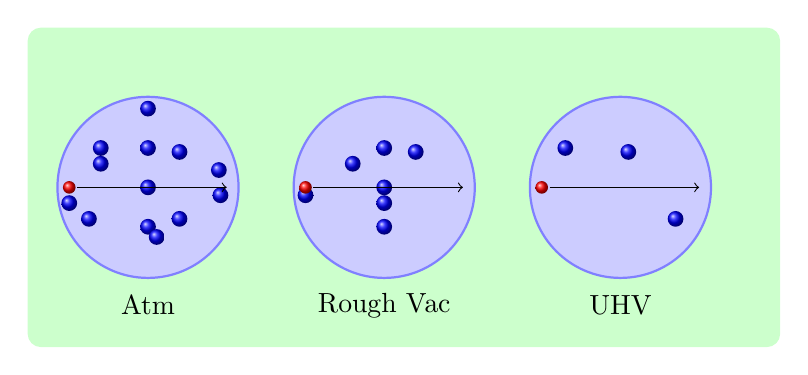
\begin{tikzpicture}[scale=1.0]
   
 \tikzstyle{vessel}=[circle,draw=blue!50,fill=blue!20,thick,
inner sep=0cm,minimum size=2.3cm]




\draw [fill=green!20,ultra thick,green!20,rounded corners] (-1.5,-2) rectangle (8,2);

\node[vessel] (V_ATM) {};
\node[vessel] (V_RV) [node distance=3cm,right of=V_ATM] {};
\node[vessel] (V_UHV) [node distance=3cm,right of=V_RV] {};

\node (ATM)[node distance=1.5cm,below of=V_ATM] {Atm};
\node (rv)[node distance=1.5cm,below of=V_RV] {Rough Vac};
\node (uhv)[node distance=1.5cm,below of=V_UHV] {UHV};

% First Vessel Molecules
\shade[ball color=blue] (0,.5) circle (.1cm);
\shade[ball color=blue] (.4,.45) circle (.1cm);
\shade[ball color=blue] (.9,.22) circle (.1cm);
\shade[ball color=blue] (-.6,.5) circle (.1cm);
\shade[ball color=blue] (-1.0,-.2) circle (.1cm);

\shade[ball color=blue] (0,-.5) circle (.1cm);
\shade[ball color=blue] (.11,-.63) circle (.1cm);
\shade[ball color=blue] (-0.75,-.4) circle (.1cm);
\shade[ball color=blue] (0,0) circle (.1cm);

\shade[ball color=blue] (-.6,.3) circle (.1cm);
\shade[ball color=blue] (.4,-.4) circle (.1cm);
\shade[ball color=blue] (0,1.0) circle (.1cm);
\shade[ball color=blue] (.92,-.1) circle (.1cm);


% Second Vessel Molecules

\shade[ball color=blue] (3,.5) circle (.1cm);

\shade[ball color=blue] (3.4,.45) circle (.1cm);

\shade[ball color=blue] (3.0,-.2) circle (.1cm);

\shade[ball color=blue] (3,-.5) circle (.1cm);

\shade[ball color=blue] (3,0) circle (.1cm);

\shade[ball color=blue] (2.6,.3) circle (.1cm);

\shade[ball color=blue] (2,-.1) circle (.1cm);




% Second Vessel Molecules

\shade[ball color=blue] (5.3,.5) circle (.1cm);

\shade[ball color=blue] (6.1,.45) circle (.1cm);




\shade[ball color=blue] (6.7,-.4) circle (.1cm);




% Beam 
\shade[ball color=red] (-1,0) circle (.08cm);

\shade[ball color=red] (2,0) circle (.08cm);

\shade[ball color=red] (5,0) circle (.08cm);
% Beam Path
\draw[->] (-0.9,0)--(1,0);

\draw[->] (2.1,0)--(4,0);

\draw[->] (5.1,0)--(7,0);

\end{tikzpicture}

\end{center}

		
\textbf{To move a particle in straight line over a long distance.}

\end{frame}







\begin{frame}{Particle Flux}
Rate of gas striking a surface or an imaginary plane of unit area.
    \begin{center}
   			\includegraphics[width=0.9\textwidth]{ParticleFlux.png}
  	 \end{center}

\begin{exampleblock}{}
Particle flux is helpful in understanding gas flow, pumping, adsorption and desorption processes.
\end{exampleblock}


\end{frame}









\begin{frame}{• Vacuum Establishment}

\begin{exampleblock}

\begin{enumerate}

\item Removal of gas molecules do not happen automatically. To establish vacuum molecules are pumped out of the vacuum system.
\item A vacuum pump is a device which removes gas molecules from the vacuum chamber. 
\item Removal of the gas molecules are done by 
\begin{itemize}
 \item Driving out molecules from the system.
 \item Absorbing molecules in a trap.
 \item Chemically changing the molecules.
\end{itemize}
 
\item Based on these principles different types of vacuum pumps are built.

\end{enumerate}

\end{exampleblock}		


\end{frame}




\begin{frame}{• Gas flow and Throughput}

\begin{center}


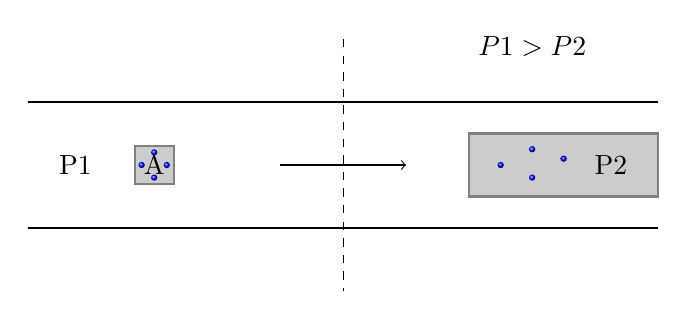
\begin{tikzpicture}[scale=0.8]
   

\draw (0,1)--(10,1);
\draw (0,-1)--(10,-1);


\draw[dashed] (5,2)--(5,-2);

\tikzstyle{rect}=[rectangle,draw=black!50,fill=black!20,thick]
\tikzstyle{rect1}=[rectangle,draw=black!50,fill=black!20,thick]
\node (gasa) at ( 2,0) [rect] {A};
\shade[ball color=blue] (2,0.20) circle (.05cm);
\shade[ball color=blue] (2,-0.20) circle (.05cm);
\shade[ball color=blue] (1.8,0) circle (.05cm);
\shade[ball color=blue] (2.2,0) circle (.05cm);
\node [node distance=1.0cm,left of=gasa] {P1};
\draw[->] (4,0)--(6,0);
\node (gasb) at ( 8,0)  {A'};
\draw [rectangle,draw=black!50,fill=black!20,thick] (7,-0.5) rectangle (10,0.5);
\node [node distance=1.0cm,right of=gasb] {P2};
\shade[ball color=blue] (8,0.25) circle (.05cm);
\shade[ball color=blue] (8,-0.20) circle (.05cm);
\shade[ball color=blue] (7.5,0) circle (.05cm);
\shade[ball color=blue] (8.5,.1) circle (.05cm);

\node [node distance=1.5cm,above of=gasb] {$P1>P2$};

%\draw (0,0) rectangle (0.5,0.5) {A};

\end{tikzpicture}
\end{center}
\textbf{Throughput(Q)} is defined as the quantity of gas flow rate, that is, the volume of gas at a known
pressure passing a plane in a known time. 
\begin{center}
$  Q=\dfrac{d(PV)}{dt}=\dfrac{d(nRT)}{dt} \Rightarrow  Q \propto \dfrac{d(n)}{dt} $ 
\end{center}

In SI unit, [Q] = $ Pa m^3  $ per second ( = 7.5 Torr liter/s) \break
Interesting Point: $ Pa-m^3 /s = N-m/s = J/s = Watt $ !


\end{frame}


\begin{frame}{• Gas Flow}

\begin{enumerate}

\item While pumping down from atmosphere, the gas in the system goes through various flow regimes. These regimes depend on the size of vacuum components, the gas species and the temperature.
\item Knudsen Number ($k_{n}$) is dimensionless quantity defined as:         
\begin{center}
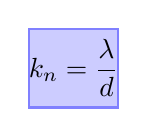
\begin{tikzpicture}[scale=0.5]
\tikzstyle{eqnbox}=[rectangle,draw=blue!50,fill=blue!20,thick,
inner sep=0cm,minimum size=1.0cm]
\node[eqnbox] (knudsen) {$k_{n}=\dfrac{\lambda}{d} $};
\end{tikzpicture}
\end{center}

 $\lambda$ = mean free path ,  d = Dimension of Vessel

\item Type of flow is defined by $k_{n}$
   \begin{itemize}
   \item When $k_{n}< 0.1$ flow is Viscous.
   \item When $ 1>k_{n}> 0.01 $ flow is Transition.
   \item When $ k_{n}> 1.0 $ flow is Molecular.
   \end{itemize}
   

\end{enumerate}

		


\end{frame}


\begin{frame}{• Viscous Flow}

\begin{center}
   			\includegraphics[width=0.25\textwidth]{ViscousFlow.png}
\end{center}





\begin{exampleblock}{Viscous Flow is like "Mob Mentality"}
 
	\begin{itemize}
	\item  The type of gas flow occurs when gas molecules are so close that there are constant collisions.
	\item  Momentum transfer between the gas molecules takes place.
    \item  Mean free path is relatively short.
    \item  Gas flows like a liquid from high pressure to lower pressure
    \item  Predominantly in the rough vacuum regime

	\end{itemize}
	


\end{exampleblock}

		


\end{frame}




\begin{frame}{Molecular Flow}

\begin{center}
   			\includegraphics[width=0.25\textwidth]{MolecularFlow.png}
   			\includegraphics[width=0.25\textwidth]{MolecularFlow1.png}
\end{center}





\begin{exampleblock}{Molecular Flow: “loner mentality”}
 
	\begin{itemize}
	\item  This type of gas flow that occurs when gas molecule's direction of movement is completely random (not necessarily from high pressure to lower pressure).
	\item  There are few collisions between molecules in the chamber.
    \item Oil molecules will Backstream (move up the rough line) in this flow regime
	\end{itemize}
	


\end{exampleblock}

		


\end{frame}

\begin{frame}{Viscous and Molecular Flow Diagram}

\begin{center}
   			\includegraphics[width=0.8\textwidth]{vismoldiagram.pdf}
   			
\end{center}

\end{frame}



\begin{frame}{Gas Flow Regime Conductance and Hardware Selection}

Vacuum hardware selection is dependent on flow regime.
\begin{enumerate}
\item Viscous Flow
	\begin{itemize}
	\item  Displacement pumps:  Rotary vane, Roots, Diaphragm
	\item  Direct pressure gauges:  Manometers, Bourdon Tubes
    \item  Elastomer seals
    \item  Less limited by the conductance of the system

	\end{itemize}
	

\item Molecular Flow

    \begin{itemize}
	\item  momentum transfer or entrapment pumps:  turbo, ion, cryo
	\item  indirect pressure gauges:  ion gauges
    \item  metal seals
    \item  VERY limited by the conductance of the system

	\end{itemize}



\end{enumerate}

		


\end{frame}









\begin{frame}{Gas Conductance}

The flow of gas in a duct or pipe depends on the pressure differential, as well on the connection geometry
	
	\begin{center}
		\includegraphics[width=0.4\textwidth]{Conductance.png}	
	\end{center}
\textbf{Conductance(C)} is defined as ratio of throughput to pressure differntial. \break

\begin{center}
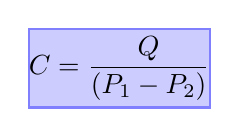
\begin{tikzpicture}[scale=0.5]
\tikzstyle{eqnbox}=[rectangle,draw=blue!50,fill=blue!20,thick,
inner sep=0cm,minimum size=1.0cm]
\node[eqnbox] (conductance) {$C=\dfrac{Q}{(P_{1}-P_{2})} $};
\end{tikzpicture}
\end{center}


\end{frame}

\begin{frame}{Conductance}

It is the capacity of a tube to allow a volume of gas pass from one end to another in unit time.
Less formally conductance is how easily gas is drawn through a vacuum component (pipe, valve, etc.)

\begin{block}

 	\begin{itemize}
		\item Conduction is dependent on type of flow.
		\item Conductance is dependent on Diameter and length.
		\item Conductance is dependent bending in piping.
   	    \item  Conductance Units:  volume/time liters/second
   		\item  Conductance can be the LIMITING factor in a pumping system.

	\end{itemize}

\end{block}
   


\end{frame}


\begin{frame}{Dependence of Conductance-1}
 
 \begin{block}{Conductance is dependent on flow}
 	\begin{center}
		
		\includegraphics[width=0.7\textwidth]{CondVsPressureCurve.png}
		
	\end{center}
\end{block}
\end{frame}


\begin{frame}{Dependence of Conductance-2}
 
 \begin{block}{Conductance is dependent on Geometry}
 	
 	\begin{center}
 	
 	
 	\begin{tabular}{ | l | l | l | }
    \hline
    Geometry & Conductance(Viscous) & Conductance(Mol)\\ \hline
   
    Aperture
    & $20A $ A area in $cm^2$
    &  $11.6A $ A area in $cm^2$ \\ \hline
	
	
    Tube(Long)
    & $ 4.97 \dfrac{D^4}{L}p_{a} $ m3/hr
    & $ 12.1 \dfrac{D^3}{L} $ l/s \\ \hline 
    
    
    
    
    
    %\hline
    \end{tabular}
\end{center}	
\end{block}
\end{frame}

\begin{frame}{Dependence of Conductance-3}
Conductance is dependent bending in piping.
\begin{center}
\includegraphics[width=0.7\textwidth]{MolFlowPipe.png}
\end{center}
\begin{block}{Transmission Probability}
 	
 	Define transmission probability, $ \alpha$ , of a duct as the ratio of the flux of gas molecules at the exit aperture to the flux at the inlet aperture $ \alpha = \dfrac{J_{Out}}{J_{In}}$  Then, in general, the conductance, C, of the duct is given by $C_A = \alpha C$  Where $C_A $ is the conductance of the entrance aperture. In molecular flow region , transmission probability determines the conductance.
 	
 		

  \end{block}
\end{frame}


\begin{frame}{Dependence of Conductance-4}
 
 \begin{block}{Conductance of complex Geometry}
 	
 	All practical vacuum structures are  complex geometrical structures , such as bend elbow etc. No standard formula exists and 
 	best possible alternative to carry out monte carlo simulation. One of the most widely used package is known as MOLFLOW , developed by 
 	CERN vacuum group scientist Dr. Karsevan and freely downloadable.
 	 \begin{center}
		
		\includegraphics[width=0.8\textwidth]{Montecarlo.png}
		
	\end{center}
 	
 		

  \end{block}
\end{frame}






\begin{frame}{Conductance for Different Types of Connection}

 \begin{exampleblock}{Series Connection}
   \begin{center}
		
		\includegraphics[width=0.8\textwidth]{SeriesConnection.png}
		
	\end{center}
\end{exampleblock}
	
\begin{exampleblock}{Parallel Connection}
	 \begin{center}
		\includegraphics[width=0.8\textwidth]{ParalleConnnection.png}
	\end{center}
\end{exampleblock}


\end{frame}




\begin{frame}{Conductance-Maximum or Minimum}

Obviously, in most cases, we want to maximize conductance.
But sometimes, we DO want to limit conductance:
Slow pumping to minimize pressure “shock” to the system.
Throttling to maintain desired pressure in system.



\end{frame}

\begin{frame}{Pumping Speed}

Pump speed: Volume of gas taken in by the pump per unit time at the pressure of the pump inlet:

                      \begin{center}
                      $ S = \dfrac{dv}{dt} $ (in lit/sec)
                      \end{center}                              
                                


Pumping Speed:  the rate at which a vacuum pump removes gasses from a system. Also known as volumetric flow rate.


Pumping Speed Units:  volume per unit time  liters per second or cubic foot per minute (CFM)

Pumping Speed and Conductance are NOT synonymous
Conductance is a property of  a component in a vacuum system.
Pumping Speed refers to the flow of gas across a plane in a system.



\end{frame}


\begin{frame}{Effective Pumping Speed}
Effective pumping speed is the net pumping speed at the outlet port of the chamber.This value is less than the pumping speed if there is a component in series between the chamber and the pump.


   \begin{center}
		
		\includegraphics[width=0.8\textwidth]{EffectivePumpingSpeed.png}
		
	\end{center}

If pumping speed is $S$ conductance of pipe in series is $ C $ and effective pumping speed is $ S^{*}$ then $ S^{*}=\dfrac{CS}{(C+S)}$



\end{frame}


\begin{frame}{Real World Connection}

Pump Speed 500 l/sec.Conductance of long round pipe $ 12 \dfrac{D^3}{L}$ D and L is in cm
 \begin{center}
		
		\includegraphics[width=0.1\textwidth]{PumpPipe.png}
		
	\end{center}

\begin{center}
 	
 	
 	\begin{tabular}{ | l | l | l | l|}
    \hline
    Pipe Dia & Length & Pipe Cond  & $S_{Eff}$ \\ \hline
   
    15 cm
    & 20 cm 
    &  2025 l/s 
    & 401 l/s \\ \hline
	
	10 cm
    & 20 cm 
    &  600 l/s 
    & 273 l/s \\ \hline
    
    %\hline
    \end{tabular}
\end{center}	


\alert{Pump is costly but pipe is cheap}


\end{frame}




\begin{frame}{Real World Connection}

 \begin{center}
		
		\includegraphics[width=0.4\textwidth]{PumpVesselConnection.png}
		
	\end{center}




\end{frame}


\begin{frame}{Vacuum Calculation-1}

 \begin{center}
		\includegraphics[width=0.8\textwidth]{VacuumCalculation1.png}
	\end{center}
\end{frame}


\begin{frame}{Vacuum Calculation-2}

 \begin{center}
		\includegraphics[width=0.8\textwidth]{VacuumCalculation2.png}
	\end{center}
\end{frame}


\begin{frame}{Vacuum Calculation-3}

 \begin{center}
		\includegraphics[width=0.8\textwidth]{VacuumCalculation3.png}
	\end{center}
\end{frame}




\begin{frame}{Pump Down Time}
\textbf{At steady state throughput is same throughout the vacuum system.}

$\dfrac{d}{dt}(pv)=-sp $ equation for throughput. \break
$\dfrac{dp}{dt}=-\dfrac{s}{v}p $ \break
$P=P_{0}exp(-\dfrac{t}{\tau})  $ where $ \tau=\dfrac{v}{s} $

\begin{exampleblock}

V = 1000 litre,
S = 500 litre/sec,
$\tau$ =2 sec
$ \Rightarrow $ every $2.3 \tau $ sec $ 10X$ pressure drop.
\end{exampleblock}


\end{frame}

\begin{frame}{Pumpdown Curve}


\begin{center}
		\includegraphics[width=0.4\textwidth]{Pumpdown1.png}
		\includegraphics[width=0.4\textwidth]{Pumpdown2.png}
	\end{center}

\end{frame}


\begin{frame}{Pumpdown Curve}

\begin{center}
   			\includegraphics[width=0.5\textwidth]{PD.png}
   			
\end{center}
$P=P_{0}exp(-\dfrac{t}{\tau})  $ is valid for only volume flow. When Surface phenomena is taken into account then 
$P=P_{0}exp(-\dfrac{t}{\tau})+\dfrac{Q_{O}}{S} +\dfrac{Q_{D}}{S} +\dfrac{Q_{P}}{S} $ where $Q_{O},Q_{D},Q_{P}$ are gas throughput by outgassing , diffusion and permeation.
\end{frame}


%\begin{frame}{Pumpdown Curve}

%\begin{center}
   		%	\includegraphics[width=0.8\textwidth]{Pumpdown.pdf}
   			
%\end{center}

%\end{frame}























%\begin{frame}
%\begin{thebibliography}{10}
%\bibitem{Goldbach1742}[Goldbach, 1742]
%Christian Goldbach.
%\newblock A problem we should try to solve \break before the ISPN ’43 deadline,
%\newblock \emph{Letter to Leonhard Euler}, 1742.
%\end{thebibliography}

%\begin{block}{Open Questions}
%Is every even number the sum of two primes?
%\cite{Goldbach1742}
%\end{block}
%\end{frame}









\end{document}